%Stand: 31.08.2017

\documentclass[ngerman]{report}

\usepackage{BiVa}
\usepackage{mathmacros}
\usepackage{figures/tikz_pictures}
\usepackage{caption}
\usepackage{listings}
\usepackage{stmaryrd}




\begin{document}

%%% tables and lists
\listoftodos
%\tableofcontents
%\listoftheorems

\chapter{1.Overview}

\begin{itemize}
	\item \enquote{image society} (webpages: 1995 text-based, 2005 image based, 
		2015 video based \dots)
		\begin{itemize}[-]
			\item data transfer rates $\uparrow$, compression rates $\uparrow$ 
			\item [critical shift: reading $\to$ watching]
		\end{itemize}
	\item \enquote{Photoshop}-ing \hfill (remove wrinkles, bumps, \dots)
	\item Images in medicine (\enquote{medical image proscessing}), x-ray, CT,
		MRI, ultrasound, \dots (\enquote{modalities}).\\
		different questions:
			\begin{enumerate}[1.)]
			  \item%
				\todoLayout{align bottom}
				\begin{minipage}{0.5\linewidth}
					measurments $\df[?]$ image\\
				  expl: tomography 	\\
					$\df$ difficult mathematical problems
				\end{minipage}
						\begin{minipage}{0.5\linewidth}
							
\begin{tikzpicture}[scale=0.5]
								\draw[help lines] (0,0) grid (3,3);
							\end{tikzpicture}
						\end{minipage}
				\item Image enhancements				
				\begin{itemize}

					\item denoising
						\begin{itemize}[]
							\item simple pixels/lines: 
							\todoWhat[so richtig?]
								\enquote{sandpaper} interpolation 
						  \item	global noise: smoothing		
						\end{itemize}

					\item grayscale
						\begin{itemize}[]
							\item histogramm balancing 
								(spreading)
						\end{itemize}

					\item distortion
						\begin{itemize}[]
							\item makes straight lines (in real world) straight 
								(in the images)
						\end{itemize}

					\item edge detection
						\begin{itemize}[]
						  \item contour enhancement 
						\end{itemize}

					\item segmentation
						\begin{itemize}[]
						  \item detect and separate parts of the image 
						\end{itemize}
					\item registration
						\begin{itemize}[]
						  \item \emph{sequence} of images of the same object 
								$\df$ \todomp{Wort?}, compare
								\begin{minipage}{0.3\linewidth}
									\todoSketch
								\end{minipage}
								$\nearrow$ object following in a movie
						\end{itemize}
				\end{itemize}
			\end{enumerate}
\end{itemize}

\textbf{\underline{Our Focus:}}
\begin{itemize}[-]
  \item mathematical models/methods/ideas 
	\item (algorthms)
	\item ((implementation))
\end{itemize}

\todoKom{skipped: Very fast intro: Matlab and images }	



\chapter{2.What is an image?}
\section{Discrete and continuous images}
There are (at least) two different points of view:
%%%%%%%%%%%%%%%%%%%%%%%%%%%
\def\leni{0.1\linewidth}
\def\lenii{0.45\linewidth}
\def\leniii{0.45\linewidth}
%%%%%%%%%%%%%%%%%%%%%%%%%%%

\begin{minipage}{\leni}
~	
\end{minipage}
\begin{minipage}{\lenii}
	$\bullet$ discrete/digital

	\begin{tikz}
		\draw[help lines] (0,0) grid (6,4);
	\end{tikz}
\end{minipage}
\begin{minipage}{\leniii}
	$\bullet$ continuous/analogue

	\begin{tikz}
		\draw[help lines] (0,0) grid (6,4);
	\end{tikz}
\end{minipage}

\begin{tabular}{p{\leni} p{\lenii} p{\leniii}}
	\textbf{object:} & matrix 															  & function \\
	\textbf{tools:}  & linear algebra (SVD, \dots) 					  & analysis (differentrage, integrate, 
		\dots) \\
	\textbf{pros:}   & (finite storage) storage, complexity   & freedom, tools,
		\todomp{motions?P.4} \par(e.g. edge discontinuity)\\
	\textbf{cons:}   & limitations: zooming, rotations, \dots & storage (infinite amout of data)\\
\end{tabular}

~\par
arguably, one has:

	\begin{itemize}
	  \item real life $\df$ continuous \enquote{images} (objects) 
		\item digital camers $\df$ discrete images
	\end{itemize}	

In general we will say:
\begin{definition}[(mathematical) image]
	A (mathematical) \emph{image} is a function	
		$$ u: \Omega \to F,$$
	\begin{tabbing}
	where: \= $\Omega \subset \Z^d$ (discrete) or $\Omega\subset \R^d$ (continuous) 
						\dots \emph{domain}\\
				 \> $d = 2$ (typical case 2D), $d=3$ (\enquote{3D image}=body or 
				 		$\underbrace{\text{2D+time}}_{\text{movie}}$)\\
				 \> $d = 4$ (3D + time) \par
	\end{tabbing}
	
	\begin{tabbing}
		$F$ \dots \= \emph{range of colours}\\
							\> $F= \R$ or $[0,\infty]$ or $[0,1]$  or $\set{0,\dots 255}$, \dots
								grayscale (light intensity) \\
							\> $F\subset \R^3$ \dots RGB image (colored)\\
							\> $F = \set{0,1}$ \dots black/white \hspace{2em}
							\begin{minipage}[c]{0.4\linewidth}
								\tikzpictureFourThree[scale=0.5]
							\end{minipage}
							\begin{minipage}[c]{0.3\linewidth}
								3 Layers\\
								$\df$ colored images:w
							\end{minipage}
	\end{tabbing}

\end{definition}

\todoKom{Matlab stuff}

Large parts of the course: analytical approach (i.e. continuous domain $\Omega$)\\
Since we want to differentirate, \dots the image $u$.
\begin{itemize}[]
  \item[Still:] need to assume that also $F$ ist continuous 
		(not as $\set{0,1}$, $\set{0,1,\dots,255}$ or $\N$)\\
		since otherwise the only differentiable (actually, the only continuous)
		functions $u: \Omega \to F$ are \emph{constant} functions 
		$\aq$ single-colour images
	\item[Also:] We usually take $F$ one-dimensional $(F \subset \R)$. 
		Think of it as either
			\begin{itemize}[-]
			  \item gray scaled image, or
				\item treating R,G \& B layer separately
			\end{itemize}
\end{itemize}

\section{Switching between discrete and continuous images}

\textbf{\large continuous $\to$ discrete:}\\
\begin{itemize}
  \item divide the continuous image in small squared pieces (boxes) 
	(superimpose grid) 

		\begin{minipage}[b]{0.6\linewidth}
		\hspace{-1em}$\bullet\;\:$now: represent each box by \emph{one} 
			value
			\begin{enumerate}[- str{a}tegy 1:]
			  \item take function value $u(x_i)$ \\
					\hspace{4em} for $x_i =$ midpoint of box $B_i$ 
				\item use mean value
					$$ \frac{1}{|B_i|}\int_{B_i} u(x) dx$$
			\end{enumerate}
		\end{minipage}%
		\begin{minipage}[t]{0.4\linewidth}
			\raisebox{1em}{\tikzpictureFIVEONE}
		\end{minipage}
\end{itemize}
$\df $ discrete image
\begin{enumerate}[str{a}tegy 1:]
  \item simple (and quick) but problemativ 
		($u(x_i)$ might represent $u|_{B_i}$ badly; 
		for $u\in L^p$, single point evaluation not
		even defined)
	\item more komplex but also more \enquote{democratic} 
		(actually closer to the way how CCD Sensors in 
		digital camers work)
\end{enumerate}
often the image value of the box $B_i$ gets also digitized, i.e.
fitted (by scaling \& rounding) into range $\set{0,1,dots,255}$
~\\
\par
\textbf{\large discrete $\to$ continous }\\

This is of course more tricky \dots

\begin{tabbing}
$\bullet$ Question:  $\quad$\= \kill

$\bullet$ Again: \> each pixel of the discrete image 
	 corresponds to a \enquote{box} of the continuous image \\
	\> (that is still to be constructed) \\

$\bullet$ Usually: \> pixel value $\mapsto$ \= function value at
	the \emph{midpoint} of the box \\
$\bullet$ Question: \> How to get the other function values 
	(in the box)?
\end{tabbing}

\hspace{1em}
\begin{minipage}[t][2cm][t]{0.30\textwidth}
	\tikzpictureSIXONE	 
\end{minipage}%
\begin{minipage}[c][2cm][t]{0.55\textwidth}
	\begin{tabbing}
 		\underline{idea 1:} $\;$ \= just take the function value of the 
			nearest\\ 
			\> midpoint (\enquote{nearest neighbour interpolation}) 
	\end{tabbing}
\end{minipage}
\vspace{-2.5em}
\begin{center}
For each $x\in B_i: u(x) := u(x_j) \;$ 
where $\displaystyle |x-x_j| = \min_{k} |x-x_k|$
\end{center}
\vspace{-.5em}
%
\begin{minipage}{0.3\linewidth}
 \tikzpictureSIXTWO
\end{minipage}
%
\begin{minipage}{0.7\linewidth}
		$\df \quad$ $u(x) = u(x_i)$ for all $x\in B_i$\\
		$\df \quad$ each box is uni-color\\
		$\df \quad$ the continuous image is essentially still discrete
\end{minipage}
~\\
~\\
{\underline{idea 2}: (bi-) lineare interpolation}



\chapter{3.Histogramm and first applicatsion}

\chapter{4.Basic Morphological Operations}

\chapter{5.Entrauschen: Filter und Co}

%\chapter{6.Kantenerkennung}

%\chapter{7.Schärfen und Entfalten}

%\chapter{8.Restauration und Inpainting}

%\chapter{9.Segementierung}

\newcommand{\quo}[1] {
\glqq #1 \grqq
}

Dieses ist die Zerlegung eines Bildes in verschiedene Objekt.\\
Eine einfach methode hierfür ist das \mim{Historgramm thresholding}:
\begin{center}
  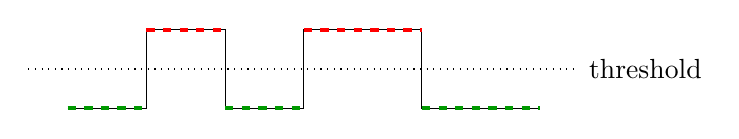
\begin{tikzpicture}
    \draw (1,0) -- (2,0) -- (2,1) -- (3,1) -- (3,0) -- (4,0) -- (4,1) -- (5.5,1) -- (5.5,0) -- (7,0);
    \draw[dotted] (0.5,0.5) -- (7.5,0.5) node[right] {threshold};
    \draw[line width=0.5mm,red,dashed] (2,1) -- (3,1);
    \draw[line width=0.5mm,red,dashed] (4,1) -- (5.5,1);
    \draw[line width=0.5mm,green!60!black,dashed] (1,0) -- (2,0);
    \draw[line width=0.5mm,green!60!black,dashed] (3,0) -- (4,0);
    \draw[line width=0.5mm,green!60!black,dashed] (5.5,0) -- (7,0);
  \end{tikzpicture}
\end{center}
So kann ein Bild in mehrere Objekte zerlegt werden.\\
Hierbei können jedoch diverse Probleme auftreten, die durch preprocessing vermindert werden sollten. Einige der preprocessing methoden sind:
\begin{enumerate}
  \item[-] Entrauschen $\nearrow$ 5.7
  \item[-] Farbraum optimal ausnutzen $\nearrow$ 3.2
  \item[-] \mim{Beleuchtungsausgleich}
\end{enumerate}
Dieser Beleuchtungsausgleich wurde nohc nicht vorher besprochen, das Problem:

\begin{center}
  \begin{tikzpicture}
    \draw (0,0) -- ++(20:1) -- ++(0,1) -- ++(20:1) -- ++(0,-1) -- ++(20:1) -- ++(0,1) -- ++(20:1.5) -- ++(0,-1) -- ++(20:1.5);
    \draw[dotted] (-0.5,1.5) -- (6,1.5) node[right] {threshold??};
  \end{tikzpicture}
\end{center}

Anstatt eines \quo{geraden} Bildes ist das Bild, etwa durch Beleuchtung, \quo{gekippt} und der Ansatz mittels Histogramthresholding würde nicht das gewünschte Ergebniss erzielen.\\

In 2D könnte dies so aus sehen.

\begin{center}
  \begin{tikzpicture}
    \draw[white] (0,0) rectangle node[draw,black] {\includegraphics[scale = 0.2]{images/Bild3plusgrad.png}} (3,3);
    \draw (1.5,3) node[above] {\LARGE $f$};
    \draw (1.5,0) node[below] {gegeben};
    \draw (3.5,1.5) node[] {\LARGE $=$};
    \draw[white] (4,0) rectangle node[draw,black] {\includegraphics[scale = 0.2]{images/Bild3.png}} (7,3);
    \draw (5.5,3) node[above] {\LARGE $u$};
    \draw (5.5,0) node[below] {erwünscht};
    \draw (7.5,1.5) node[] {\LARGE $+$};
    \draw[white] (8,0) rectangle node[draw,black] {\includegraphics[scale = 0.2]{images/Bild3grad.png}} (11,3);
    \draw (9.5,3) node[above] {\LARGE $v$};
    \draw (9.5,0) node[below] {gesucht};
    \draw (11.75,1.5) node[] {\LARGE $\Longleftrightarrow$};
    \draw[white] (12.5,0) rectangle node[draw,black] {\includegraphics[scale = 0.2]{images/Bild3thresh.png}} (15.5,3);
    \draw (14,3) node[above] {};
    \draw (14,0) node[below] {Ergebnis durch thresholding};
  \end{tikzpicture}
\end{center}

Rechts ist das Bild, das durch das Beschreibene Histogramm thresholding dargestellt wurde zu sehen. Methoden um durch preprocessing den gesuchten Gradienten zu entfernen werden im folgenden beschrieben.

\section{Beleuchtungsausgleich}

\begin{enumerate}
  \item[Einfachster Fall:] $v$ konstant. In diesem Fall kann man etwa eine \quo{Leeraufnahme} machen, $v=f$ setzen und dieses $v$ in allen folgenden Aufnahmen subtrahieren.
  \item[Normalfall:] $v$ ändert sich bei Jeder Aufnahme. Hierbei gibt es mehrere Ansätze:
\end{enumerate}

\begin{enumerate}
  \item[a)] \mim{Lineare Regression}: \\
  \begin{minipage}[c]{0.6\linewidth}
          \item[] Wir Unterstellen das der Verlauf \mim{affin-linear} ist, d.h.:
          \[v(x,y) = a x + b y + c\]
          Diese Parameter $a$, $b$, $c$ gilt es nun zu schätzen. 
    \end{minipage}
    \hfill
    \begin{minipage}[c]{0.35\linewidth}
              \begin{center}
        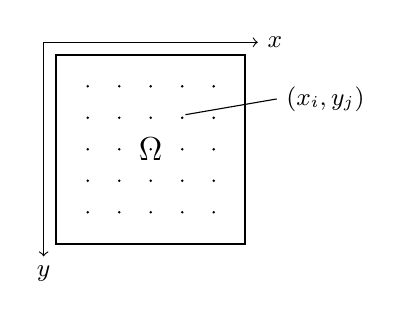
\begin{tikzpicture}[scale=0.8]
          \draw[thick] (0,0) rectangle node[] {\large $\Omega$} (3,3);
          \draw[->] (-0.2,3.2) -- (3.2,3.2) node[right] {\small $x$};
          \draw[->] (-0.2,3.2) -- (-0.2,-0.2) node[below] {\small $y$};
          \foreach \x in {1,...,5}
            \foreach \y in {1,...,5}{
              \draw (\x / 2,\y / 2) node[circle,fill=black,inner sep=0pt] {};
          }
          \draw (2.05,2.05) -- (3.5,2.3) node[right] {\small $(x_i,y_j)$};
        \end{tikzpicture}
      \end{center}
    \end{minipage}
    Dazu soll gelten
    \[\forall (x,y) \in \Omega : ax+by+c \approx f(x,y)\]
    um dieses zu erfüllen wird eine Stichprobe von endlich vielen Punkten $(x_i,y_i)$ aus $\Omega$ gewählt und durch diese ein Gleichungs System gebildet.
    
    \begin{gather*} 
    ax_1+by_1+c \approx f(x_1,y_1)\\
    \vdots \\
    ax_n+by_n+c \approx f(x_n,y_n)
    \end{gather*}
    In Matrix form ergibt sich:
    
    \[\underbrace{\mat{x_1 & y_1 & 1 \\ \vdots & \vdots & \vdots \\ \vdots & \vdots & \vdots \\ \vdots & \vdots & \vdots \\ x_n & y_n & 1}}_{A} \underbrace{\mat{a \\ b \\ c}}_{w} \approx \underbrace{\mat{f(x_1,y_1 \\ \vdots \\ \vdots \\ \vdots \\ f(x_n,y_n)}}_{z}\]
    Die optimale Lösung dieses Problems kann über die \mim{Normalengleichung} berechnet werden.
    
    \[A^T A w = A^T z\]
    
    Dauraus erhält man $w$, somit auch $a$, $b$, $c$ und schlussendlich $v \Rightarrow u = f-v$.\\
    Anschließend wird noch ein Histogram stretching durchgeführt um das finale Bild zu erhalten.
    
    \item[b)] \mim{Polynomiale Regression}:
    Ähnlich zur linearen Regression nun wird hierbei keine affin-lineare Funktion, sondern ein polynom genutzt. Für ein Polynom zwieten gerades kann etwa die Funktion
    \[v(x,y) = ax^2 by^2 cxy+ dx +ey +f\]
    gewählt werden. Wieder entsteht ein Gleichungssytem:
    
    \[\underbrace{\mat{x_1^2 & y_1^2 & x_1y_1 & x_1 & y_1 & 1 \\ \vdots & \vdots & \vdots & \vdots & \vdots & \vdots \\ \vdots & \vdots & \vdots & \vdots & \vdots & \vdots \\ \vdots & \vdots & \vdots & \vdots & \vdots & \vdots \\ x_n^2 & y_n^2 & x_ny_n & x_n & y_n & 1}}_{A} \underbrace{\mat{a \\ b \\ c \\ d \\e \\ f}}_{w} \approx \underbrace{\mat{f(x_1,y_1 \\ \vdots \\ \vdots \\ \vdots \\ f(x_n,y_n)}}_{z}\]

  \item[c)] \mim{Trigonometrisches Polynom}
  Hierbei wird $v$ in den niedrigfrequenten Anteilen von $f$ gesucht.
  
  \begin{center}
    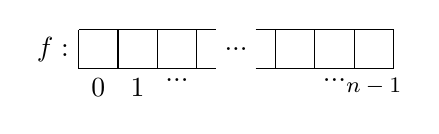
\begin{tikzpicture}
      \draw (0,0.25) node[left] {$f:$};
      \draw[step = 0.5] (0,0) grid (1.75,0.5);
      \draw (2,0.25) node[] {$...$};
      \draw[step = 0.5] (2.25,0) grid (4,0.5);
      \draw (0.25,0) node[below] {$0$};
      \draw (0.75,0) node[below] {$1$};
      \draw (1.25,0) node[below] {$...$};
      \draw (3.25,0) node[below] {$...$};
      \draw (3.75,0) node[below] {\footnotesize $n-1$};
    \end{tikzpicture}
  \end{center}
  
  Es ergibt sich $\hat f$:
  
  \[\hat f_k = \sum_{m=0}^{n-1} f_k \bigl(\underbrace{e^{- i 2 \pi \frac{k}{n}}}_{w_k}\bigr)^m \quad , \ k= 0,1,...,n-1\]
  
  Mittels der FFT (Fast Fourier Transformation) ergibt sich $\hat f$ zu:

  \begin{center}
    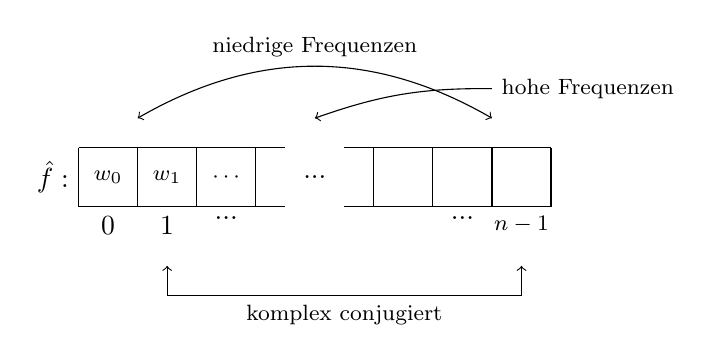
\begin{tikzpicture}[scale=1.5]
      \draw (0,0.25) node[left] {$\hat f:$};
      \draw[step = 0.5] (0,0) grid (1.75,0.5);
      \draw (2,0.25) node[] {$...$};
      \draw[step = 0.5] (2.25,0) grid (4,0.5);
      \draw (0.25,0) node[below] {$0$};
      \draw (0.75,0) node[below] {$1$};
      \draw (0.25,0.25) node[] {\footnotesize $w_0$};
      \draw (0.75,0.25) node[] {\footnotesize$w_1$};
      \draw (1.25,0) node[below] {$...$};
      \draw (3.25,0) node[below] {$...$};
      \draw (1.25,0.25) node[] {\footnotesize$\cdots$};
      \draw (3.75,0) node[below] {\footnotesize $n-1$};
      \draw[<->] (0.75,-0.5) -- (0.75,-0.75) -- node[below] {\footnotesize komplex conjugiert} (3.75,-0.75) -- (3.75,-0.5);
      \draw[<->] (0.5, 0.75) to[bend left] node [above] {\footnotesize niedrige Frequenzen} (3.5,0.75);
      \draw[<-] (2,0.75) to[bend left=10] (3.5,1) node[right] {\footnotesize hohe Frequenzen};
    \end{tikzpicture}
  \end{center}
  Durch entfernen dieser niedrigen Frequenzen ergibt sich $u$.
Ähnliches funktioniert auch in 2D:

    \begin{center}
    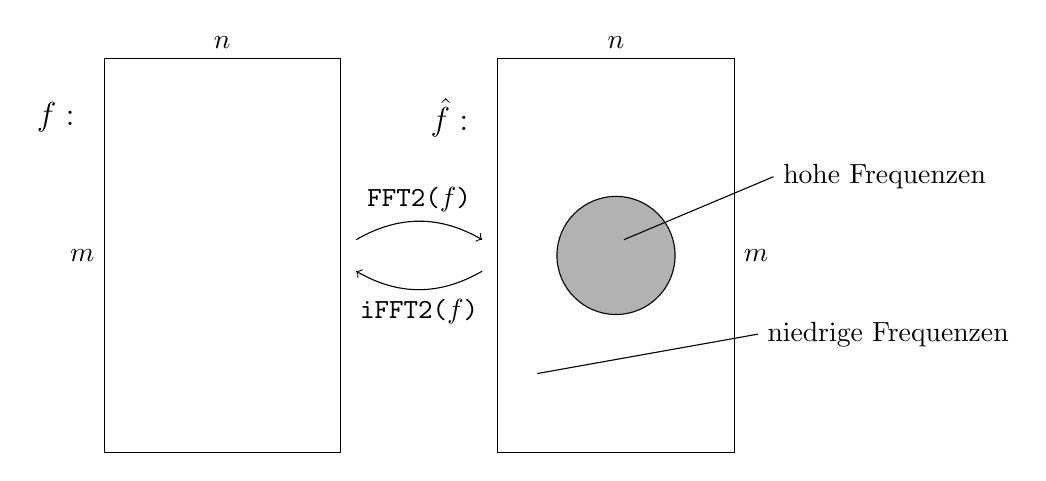
\begin{tikzpicture}[scale=1]
      \draw (0,0) rectangle (3,5);
      \draw (1.5,5) node[above] {$n$};
      \draw (0,2.5) node[left] {$m$};
      \draw (-0.25,4.25) node[left] {\large $f:$};
      \draw[->] (3.2,2.7) to[bend left] node[above] {\tt{FFT2($f$)}} (4.8,2.7);
      \draw[<-] (3.2,2.3) to[bend right] node[below] {\tt{iFFT2($f$)}} (4.8,2.3);
      \draw (5,0) rectangle (8,5);
      \draw (6.5,5) node[above] {$n$};
      \draw (8,2.5) node[right] {$m$};
      \draw (4.75,4.25) node[left] {\large $\hat f:$};
      \draw[fill = black!30] (6.5,2.5) circle (0.75);
      \draw (6.6,2.7) -- (8.5,3.5) node[right] {hohe Frequenzen};
      \draw (5.5,1) -- (8.3,1.5) node[right] {niedrige Frequenzen};
    \end{tikzpicture}
  \end{center}
\end{enumerate}

%\chapter{10.Registrierung}

%\chapter{11.Mathematischer Nachschlag}
Aus mathematischer Sicht sind einige Fragen offen geblieben, etwa:

\newcommand{\D} {
\mathcal{D}
}

\section{Verallgemeinerte Funktionen und Abbleitungen}
Wie differenziert man unstetige Funktionen?

Sei $\D := C_0^\infty(\R^d)$ die Menge (auch ein Vektorraum) der beliebig oft differenzierbaren Funktionen auf $\R^d$ mit beschränktem Träger. Etwa:

\begin{center}
    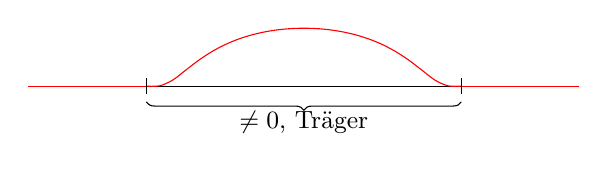
\begin{tikzpicture}
        \draw (-3,0) -- (3,0);
        \draw[scale=2,domain=-0.999:0.999,smooth,variable=\x,red] plot ({\x},{e^(-(1 - abs(\x)^2 )^(-1)});
        \draw[red] (-3.5,0) -- (-0.999*2,0);
        \draw[red] (3.5,0) -- (0.999*2,0);
        \draw (0.999*2,-0.1) -- (0.999*2,0.1);
        \draw (-0.999*2,-0.1) -- (-0.999*2,0.1);
        \draw[decorate,decoration={brace,amplitude=3pt,mirror}] (-2,-0.2) -- node[below] {\small $\neq0$, Träger} (2,-0.2);
    \end{tikzpicture}
\end{center}

Diese Funktion ist:

\[\varphi(x)=g(1- \abs{x}^2)\]

wobei

\[g(t) := \begin{cases}
    e^{\frac{-1}{t}} & ,t>0\\
    0 & ,t\leq 0
\end{cases}\]

Dieses Funktioniert auch im $\R^d$

\def\centerx{2}
\def\centery{-1}

\begin{center}
    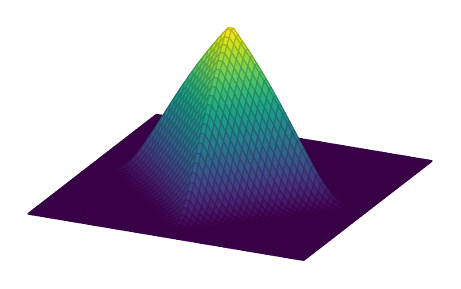
\begin{tikzpicture}[        declare function={
        func(\x) = (\x>0) * e^(-(\x)^(-1)) +
                   (\x<=0) * 0;
      }]

        \pgfplotsset{
            colormap name=viridis,
        }
            \begin{axis}[hide axis,scale=0.75,name=plot1,samples=10]
                \addplot3[surf,domain=-1:1,domain y=-1:1,samples=60]
                    {func(1 - abs(x) - abs(y)))};
                \end{axis}
    \end{tikzpicture}
\end{center}

ist $C_0^\infty(\R^d)$ und hat kompakten Träger.

Sei nun $L^1_{loc}(\R^d)$ die Menge aller Funktionen auf $\R^d$ mit kompaktem Träger für die:

\[\int_K \abs{f(x)} dx < \infty\]

für alle abgeschlossenen und beschränkten Mengen $K \subset \R^d$ gilt.

\begin{center}
    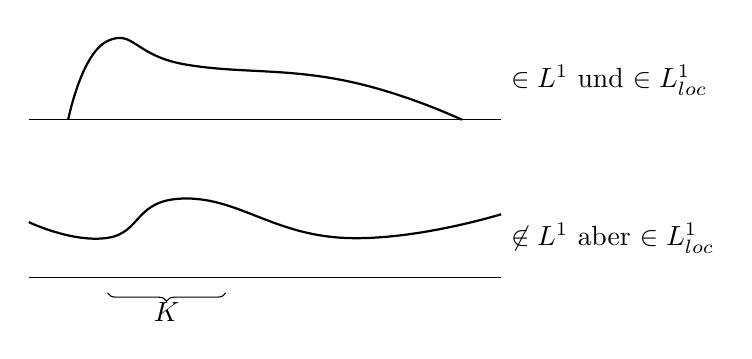
\begin{tikzpicture}
        \draw (-3,0) -- (3,0);
        \draw[thick] plot [smooth, tension = 0.8] coordinates {(-2.5,0) (-2,1)  (-1,0.7) (1,0.5) (2.5,0)};
        \draw (3,0.5) node[right] {$\in L^1$ und $\in L^1_{loc}$};
        \draw (-3,-2) -- (3,-2);
        \draw[thick] plot [smooth, tension = 0.8] coordinates {(-3,-1.3) (-2,-1.5) (-1,-1) (1,-1.5) (3,-1.2) };
        \draw (3,-1.5) node[right] {$\not \in L^1$ aber $\in L^1_{loc}$}; 
        \draw[decorate,decoration={brace,amplitude=3pt,mirror}] (-2,-2.2) -- node[below] {$K$} (-0.5,-2.2);
    \end{tikzpicture}
\end{center}

Die Zweite Funktion ist nicht in $L^1$ da ihr Gesamtintegral nicht endlich ist jedoch ist das Integral über jede endlich Menge endlich, sie hat also keine Pole, somit sie in $L^1_{loc}$.

Für jede Funktion $f \in L^1_{loc}(\R^d)$ bildet 
\begin{equation}\label{eq.11.1}
    \tilde f:\varphi \in \Omega \mapsto \int_{\R^d} f(x) \C \varphi(x) dx \in \R
\end{equation}

ein stetiges lineares Funktional auf $\D$.

Sei nun $\D'$ die Menge aller stetigen linearen Funktionale auf $\D$, also der \mim{Dualraum}. Also ist für jedes $f \in L^1_{loc}$ das Funktional $\tilde f$ aus \eqref{eq.11.1} in $\D'$.

\begin{center}
    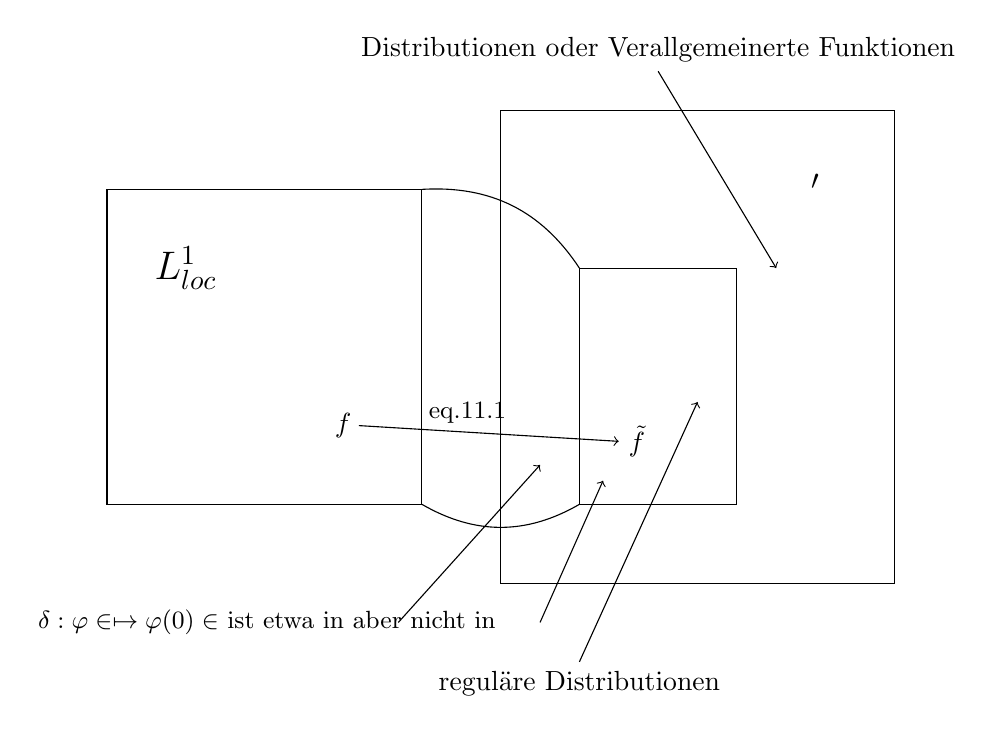
\begin{tikzpicture}
        \draw (0,0) rectangle (4,4);
        \draw (1,3) node[] {\Large $L^1_{loc}$};
        \draw (3,1) node[] {$f$};
        \draw (5,-1) rectangle (10,5);
        \draw (6,0) rectangle (8,3);
        \draw (4,4) to[bend left] (6,3);
        \draw (4,0) to[bend right] (6,0);
        \draw[->] (3.2,1) -- node[above]{\small \eqref{eq.11.1} \ \ \ \ \ } (6.5,0.8) node[right] {$\tilde f$};
        \draw (9,4) node[] {\Large $\D'$};
        \draw[<-] (7.5,1.3) -- (6,-2) node[below]{reguläre Distributionen};
        \draw[<-] (8.5,3) -- (7,5.5) node[above]{\mim{Distributionen} oder Verallgemeinerte Funktionen};
        \draw (-1,-1.5) node[right] {\small $\delta:\varphi \in \D \mapsto \varphi(0) \in \R$ ist etwa in  aber nicht in};
        \draw[<-] (6.3,0.3) -- (5.5,-1.5);
        \draw[<-] (5.5,0.5) -- (3.7,-1.5);
    \end{tikzpicture}
\end{center}

Nun zu den Abbleitungen, sein zunächst $d=1$ und $f \in C^1 \subset L^1_{loc}$, dann gilt für alle $\varphi \in \D$ wobei $[-a,a] \supset supp(\varphi)$:

\[\underbrace{\int_{\R^1} f'(x) \varphi(x) dx}_{f'(\varphi)} = \int_{-a}^a f(x) \phi(x) dx = \underbrace{f(x)\varphi(x)|_{-a}^{a}}_{=0} - \int_{-a}^a f(x) \varphi'(x) dx = -\int_{\R^1} f(x) \varphi'(x) dx = -\tilde f(\varphi')\]

$\Rightarrow$ Für $f \in C^1 \subset L^1_{loc}$ gilt $\tilde f'(\varphi) = - \tilde f(\varphi'), \varphi \in \D$. Wir nehmen dies als Ansatz und setzen:

\begin{equation}\label{eq.11.2}
    F'(\varphi):=-F(\varphi'), \varphi \in \D
\end{equation}

für alle $F\in \D$, genannt Distributionen Abbleitung.

Beispiel:

\begin{center}
    \begin{tikzpicture}
        \draw (-0.4,0) node[left] {$f(x) = \abs{x}$};
        \draw (-0.2,0) -- (4.2,0);
        \draw[thick] (0,2) -- (2,0) -- (4,2);
        \draw (2,-0.1) -- (2,2.3);
    \end{tikzpicture}
\end{center}
Und $F:=\tilde f$ also:

\[F'(\varphi) = -F(\varphi) = - \int_{-a}^a \abs{x} \varphi'(x) dx = - \int_{-a}^0 -x \varphi'(x) dx - \int_0^a x \varphi'(x) dx \]

\[= \int_{-a}^0 x \varphi'(x) dx - \int_0^a x \varphi'(x) dx = \underbrace{x \varphi(x)|_{-a}^0}_{0} - \int_{-a}^0 1 \varphi(x) dx - \underbrace{x \varphi(x)|_0^a}_{0} + \int_0^a 1 \varphi(x) dx\]

\[= \int_{-a}^a sing(x) \varphi(x) dx = \tilde{sign}(\varphi)\]

\begin{center}
    \begin{tikzpicture}
        \draw (-0.4,0) node[left] {$sign(x)=$};
        \draw (-0.2,0) -- (4.2,0);
        \draw (2,-1.3) -- (2,1.3);
        \draw[thick] (2,1) node[left]{\small $1$} -- (4,1);
        \draw[thick] (0,-1) -- (2,-1) node[right]{\small $-1$};
    \end{tikzpicture}
\end{center}

Also insgesamt $F'=\tilde{sign}$

%\clearpage
%\setcounter{page}{1}


%\appendix 

\end{document}
